\documentclass[11pt]{article}

% -------------------- Packages --------------------
\usepackage[margin=1in]{geometry}
\usepackage{microtype}
\usepackage{amsmath,amssymb,amsthm,mathtools}
\usepackage{booktabs}
\usepackage{graphicx}
\usepackage{hyperref}
\usepackage{algorithm}
\usepackage{algpseudocode}
\usepackage{enumitem}
\usepackage{tikz}
\usetikzlibrary{positioning,arrows.meta,bending}

% -------------------- Macros --------------------
\newcommand{\E}{\mathbb{E}}
\newcommand{\Var}{\mathrm{Var}}
\newcommand{\1}{\mathbf{1}}
\newcommand{\R}{\mathbb{R}}
\newcommand{\Z}{\mathbb{Z}}

\newcommand{\fall}[2]{\left(#1\right)_{#2}} % falling factorial
\newcommand{\coll}{\mathcal{C}} % collision event (avoid conflict with C matrix)

% -------------------- Theorem Environments --------------------
\theoremstyle{plain}
\newtheorem{theorem}{Theorem}
\newtheorem{proposition}{Proposition}
\newtheorem{lemma}{Lemma}

\theoremstyle{definition}
\newtheorem{definition}{Definition}

% -------------------- Title --------------------
\title{\vspace{-0.6em}
Estimating Same-Source Probabilities from Value Collisions\\
with Unknown Latent Emission Graphs
\vspace{-0.3em}}
\author{%
\textbf{Jason Bono}\\
\vspace{-0.7em}
}
\date{\vspace{-0.8em}February 2026\vspace{-0.6em}}

\begin{document}
\maketitle

\begin{abstract}
We study a measurement model in which unobserved latent entities emit observable value labels according to an unknown emission spectrum.
The spectrum is represented as a bipartite multigraph whose bottom vertices are latent entities and whose top vertices are value labels; a measurement draw samples an edge uniformly at random and returns the value endpoint.
Given two measurement draws, we ask for the posterior probability that the two observed values came from the same latent entity, especially when the observed values collide (match).
When the full emission graph is known, this posterior admits a simple closed form in terms of the incidence matrix.
The main contribution of this paper is an estimator for the collision-conditioned same-source probability when the full graph is unknown, the observer knows only the value-label marginals (value-side degrees), and the observer has domain knowledge about the \emph{variance} of entity degrees (heterogeneity of emission volume across entities).
Under a maximum-entropy (configuration-model) ensemble over bipartite multigraphs consistent with the observed value marginals, we prove that the ensemble mean of the exact posterior depends on the unknown entity side only through the entity-degree second moment, equivalently the across-entity degree variance.
We also derive an analytic expression for the ensemble variance (uncertainty) of the posterior across graphs, which depends on one additional degree-shape statistic (a third falling-factorial moment).
We validate the formulas by exact enumeration in small toy examples and by an end-to-end demonstration that samples ground-truth graphs, simulates measurements, estimates value marginals from finite data, and compares the true posterior to the mean estimate and uncertainty bands. 
\end{abstract}

\medskip
\noindent\textbf{Keywords:} same-source probability, value collision, bipartite configuration model, maximum-entropy ensemble, record linkage, entity resolution

\vspace{0.2em}

% ============================================================
\section{Introduction}
Many systems observe \emph{values} but not the \emph{entities} that produced them.
Examples include repeated measurements of latent sources, anonymized logs, records produced by hidden actors, or sensors that emit coarse labels.
Even when a value repeats (a ``collision''), it may reflect either repeated emission from the same latent entity or emissions from different entities that share common values.
Quantifying this ambiguity is useful for debugging pipelines, designing downstream inference, and understanding privacy and identifiability properties.

This paper considers a stylized but broadly applicable model: latent entities emit value labels with different intensities.
The (unobserved) emission spectrum is encoded as a bipartite multigraph with integer edge multiplicities.
A measurement draw samples an edge uniformly and returns the value label.
We focus on the simplest nontrivial question: given two draws (with replacement), what is the posterior probability that they came from the same latent entity, especially conditioned on observing a value collision?

When the full emission graph is known, the posterior is computable exactly.
The challenging regime is when the full graph is not known.
We assume the observer can estimate the value-label marginal distribution (equivalently, value-side degrees up to scale) and that domain knowledge provides a summary of entity-side heterogeneity---in this paper, the across-entity degree variance.
We then:
\begin{itemize}[leftmargin=*]
\item introduce a maximum-entropy bipartite graph ensemble (configuration model) consistent with the observed value marginals,
\item prove that the ensemble mean of the exact posterior given a collision is determined solely by the entity-degree second moment (variance),
\item derive an analytic expression for the ensemble variance (uncertainty) across graphs,
\item validate by exact enumeration in small toy examples, and
\item demonstrate end-to-end performance: sampling ground-truth graphs, simulating measurements, estimating value marginals from finite data, and comparing the true posterior to the estimator's mean and uncertainty bands.
\end{itemize}

% ============================================================
\section{Related work}
\label{sec:related}

\paragraph{Record linkage and the Fellegi--Sunter model.}
Fellegi and Sunter \cite{fellegi1969} cast record linkage as a likelihood-ratio test between a
\emph{match} hypothesis (same source) and a \emph{non-match} hypothesis (different source),
leading to the familiar $m$- and $u$-probabilities for field agreement:
$m = P(\text{agree}\mid \text{match})$ and $u = P(\text{agree}\mid \text{non-match})$.
In our setting with a single equality comparator, the ``agree'' event is exactly the collision event $\coll=\{V_1=V_2\}$.
The Fellegi--Sunter posterior for an agreement,
\[
P(\text{match}\mid \text{agree})=\frac{m\,\pi}{m\,\pi + u\,(1-\pi)},
\]
maps directly to our target $\theta(C)=P(S\mid \coll)$, with prior $\pi=P(S)$.
A key difference is that classical linkage frameworks typically treat $(m,u,\pi)$ as free parameters and
estimate them from labeled data or via EM \cite{jaro1989,winkler2006};
later statistical models refine the probabilistic foundations \cite{copas1990}.
Here we instead start from a generative emission graph model, and derive $\theta(C)$ exactly when $C$ is known
(Proposition~\ref{prop:known}), and in closed form \emph{in expectation} when $C$ is unknown under a
maximum-entropy (configuration-model) ensemble (Theorem~\ref{thm:mean}).

\paragraph{Entity resolution and duplicate detection.}
Entity resolution and duplicate detection aim to infer the full partition or matching structure among records,
often leveraging multiple noisy fields and transitive/collective constraints.
Surveys and textbooks in the database and data-mining communities emphasize the end-to-end ER pipeline,
including blocking/indexing, similarity computation, and clustering/classification
\cite{elmagarmid2007,hernandez1995,christen2012book,christen2012survey,getoor2012}.
Collective ER models exploit relational structure and dependencies across decisions
\cite{bhattacharya2007}.
Recent Bayesian approaches place priors directly on the latent partition or bipartite matching
\cite{steorts2016,sadinle2017}.
In contrast, our goal is a single scalar summary---the collision-conditioned same-source probability---and we
derive it analytically under a principled random-graph null (configuration model) consistent with observed value marginals.
This scalar can be interpreted as the \emph{precision} of an equality-based blocking key:
among colliding values, what fraction of collisions are truly same-source?

\paragraph{Collision probabilities, concentration, and the ``birthday'' phenomenon.}
The probability that two draws from a discrete distribution collide is the classical birthday problem and is
closely related to concentration indices such as Simpson's concentration (and the Herfindahl index)
\cite{simpson1949,flajolet1992birthday}.
Our setting introduces a second layer: values are generated via an unobserved bipartite emission structure,
so the same-source probability \emph{given} a collision depends on both value-side and entity-side heterogeneity.
Under the configuration-model ensemble, we show that the ensemble mean of this conditional probability depends
on the entity side only through the degree second moment (Theorem~\ref{thm:mean}).

\paragraph{Privacy and disclosure risk.}
Collisions of quasi-identifier values are central to disclosure risk: if a released key value is rare or unique,
it can enable re-identification \cite{sweeney2002}, and uniqueness of partial identifiers has been quantified in several domains.
De-anonymization attacks show that sparse/high-dimensional keys can be re-linked to individuals even without explicit identifiers
\cite{narayanan2008}.
Our $\theta(C)=P(S\mid \coll)$ addresses a complementary question to group-size metrics such as $k$-anonymity:
\emph{given that a released key value repeats, how likely is it that the repetition is due to the same individual/source rather than different individuals sharing the key?}
This provides an interpretable ``collision informativeness'' statistic that can be used for debugging linkage pipelines or
for characterizing match risk under repeated values.

% ============================================================
\section{Model and exact posteriors when the graph is known}

\subsection{Latent emission spectrum as a bipartite multigraph}
Let $e_1,\dots,e_n$ denote latent entities and $v_1,\dots,v_m$ denote value labels.
The emission spectrum is represented by a nonnegative integer incidence matrix
\[
C = (c_{ia}) \in \Z_{\ge 0}^{n\times m},
\]
where $c_{ia}$ is the number of edges between entity $e_i$ and value $v_a$.

Define entity degrees and value degrees:
\[
\ell_i := \sum_{a=1}^m c_{ia},
\qquad
o_a := \sum_{i=1}^n c_{ia},
\qquad
T := \sum_{a=1}^m o_a = \sum_{i=1}^n \ell_i.
\]
We interpret $T$ as the total number of edge ``stubs'' (total emission mass).

\subsection{Measurement draws}
A single measurement draw samples one edge uniformly at random from the multigraph and returns the value label endpoint.
Equivalently: sample an entity-value edge uniformly, observe only the value endpoint.
Consider two draws with replacement.
Let $E_1,E_2\in\{e_1,\dots,e_n\}$ be the latent emitting entities and $V_1,V_2\in\{v_1,\dots,v_m\}$ the observed values.
Define events:
\[
S := \{E_1 = E_2\} \quad\text{(same latent source)},
\qquad
\coll := \{V_1 = V_2\} \quad\text{(value collision)}.
\]

\begin{figure}[htbp]
\centering
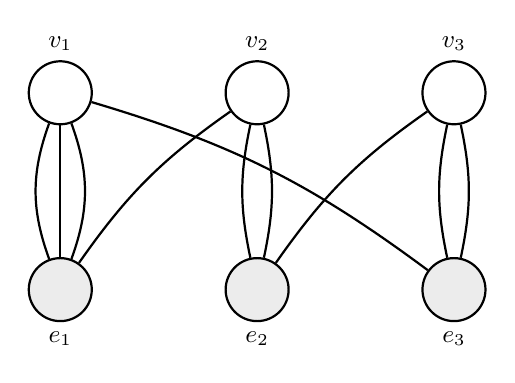
\begin{tikzpicture}[
  entity/.style={circle, draw, thick, minimum size=8mm, fill=gray!15},
  value/.style={circle, draw, thick, minimum size=8mm, fill=white},
  every label/.style={font=\small},
  node distance=2.0cm
]

% Value nodes (top row)
\node[value, label=above:{$v_1$}] (V1) at (0,  2.5) {};
\node[value, label=above:{$v_2$}] (V2) at (2.5,2.5) {};
\node[value, label=above:{$v_3$}] (V3) at (5,  2.5) {};

% Entity nodes (bottom row)
\node[entity, label=below:{$e_1$}] (E1) at (0,  0) {};
\node[entity, label=below:{$e_2$}] (E2) at (2.5,0) {};
\node[entity, label=below:{$e_3$}] (E3) at (5,  0) {};

% --- e1 -> v1: multiplicity 3 (three parallel edges) ---
\draw[thick] (E1) to[bend left=20]  (V1);
\draw[thick] (E1) --                (V1);
\draw[thick] (E1) to[bend right=20] (V1);

% --- e1 -> v2: multiplicity 1 ---
\draw[thick] (E1) to[bend left=10] (V2);

% --- e2 -> v2: multiplicity 2 (two parallel edges) ---
\draw[thick] (E2) to[bend left=12]  (V2);
\draw[thick] (E2) to[bend right=12] (V2);

% --- e2 -> v3: multiplicity 1 ---
\draw[thick] (E2) to[bend left=10] (V3);

% --- e3 -> v1: multiplicity 1 ---
\draw[thick] (E3) to[bend right=10] (V1);

% --- e3 -> v3: multiplicity 2 (two parallel edges) ---
\draw[thick] (E3) to[bend left=12]  (V3);
\draw[thick] (E3) to[bend right=12] (V3);

\end{tikzpicture}
\caption{Emission-spectrum bipartite multigraph.
Bottom nodes are latent entities ($e_1,e_2,e_3$); top nodes are value labels ($v_1,v_2,v_3$).
Each edge represents one unit of emission mass; parallel edges encode higher emission strength (e.g., $e_1$ emits $v_1$ with multiplicity~3).
A measurement draw samples one edge uniformly at random and returns the value endpoint.}
\label{fig:diagram}
\end{figure}

\subsection{Exact posteriors for a known incidence matrix}
The following identities are elementary but form the foundation for the unknown-graph analysis.

\begin{proposition}[Known-graph posteriors]
\label{prop:known}
Assume $C$ is known and draws are with replacement.
Then for any $(a,b)$ with $o_a,o_b>0$,
\[
P(S \mid V_1=v_a, V_2=v_b)
=
\frac{\sum_{i=1}^n c_{ia}c_{ib}}{o_a o_b}.
\]
In particular,
\[
P(S\mid V_1=v_a, V_2=v_a) = \frac{\sum_{i=1}^n c_{ia}^2}{o_a^2}.
\]
Conditioned only on the event of a collision,
\[
\boxed{
P(S\mid \coll)
=
\frac{\sum_{a=1}^m\sum_{i=1}^n c_{ia}^2}{\sum_{a=1}^m o_a^2}.
}
\]
\end{proposition}

\begin{proof}
For a single draw, $P(E=e_i, V=v_a)=c_{ia}/T$, hence $P(V=v_a)=o_a/T$ and
\[
P(E=e_i \mid V=v_a)=\frac{P(E=e_i,V=v_a)}{P(V=v_a)}=\frac{c_{ia}/T}{o_a/T}=\frac{c_{ia}}{o_a}.
\]
Because the two draws are independent (with replacement),
\[
P(S \mid V_1=v_a,V_2=v_b)
= \sum_{i=1}^n P(E_1=e_i\mid V_1=v_a)\,P(E_2=e_i\mid V_2=v_b)
= \sum_{i=1}^n \frac{c_{ia}}{o_a}\frac{c_{ib}}{o_b},
\]
which gives the first identity. The collision-at-$v_a$ case is $a=b$.

For the collision-only posterior, write $P(S\mid \coll)=P(S\cap \coll)/P(\coll)$.
Under with-replacement edge sampling,
\[
P(S\cap \coll)=\sum_{i=1}^n\sum_{a=1}^m P(E_1=e_i,V_1=v_a)\,P(E_2=e_i,V_2=v_a)
= \sum_{i,a}\left(\frac{c_{ia}}{T}\right)^2=\frac{\sum_{i,a}c_{ia}^2}{T^2}.
\]
Similarly,
\[
P(\coll)=\sum_{a=1}^m P(V_1=v_a)P(V_2=v_a)=\sum_a\left(\frac{o_a}{T}\right)^2=\frac{\sum_a o_a^2}{T^2}.
\]
Taking the ratio yields $P(S\mid \coll)=\bigl(\sum_{i,a}c_{ia}^2\bigr)\big/\bigl(\sum_a o_a^2\bigr)$.
\end{proof}

We will write
\[
\theta(C) := P(S\mid \coll)
=
\frac{N(C)}{D},
\qquad
N(C) := \sum_{i,a} c_{ia}^2,
\qquad
D := \sum_{a} o_a^2.
\]
When $C$ is unknown, $\theta(C)$ becomes a random variable over plausible graphs.

% ============================================================
\section{Unknown-graph regime and maximum-entropy graph ensemble}

\subsection{Observer information}
In the unknown-graph regime, the observer does not know $C$ (and typically does not know $\ell$).
We assume the observer knows:
\begin{itemize}[leftmargin=*]
\item the number of \emph{active emitters} $n$ (entities that exist and emit),
\item the value-side degrees $o=(o_1,\dots,o_m)$ (or equivalently the marginal distribution $P(V=v_a)=o_a/T$),
\item and a domain-knowledge parameter describing entity heterogeneity: the across-entity degree variance $\sigma^2$.
\end{itemize}
For active emitters, we assume $\ell_i\ge 1$ for all $i$, hence $T\ge n$.

Let
\[
\mu := \frac{1}{n}\sum_{i=1}^n \ell_i = \frac{T}{n},
\qquad
\sigma^2 := \frac{1}{n}\sum_{i=1}^n (\ell_i-\mu)^2.
\]
Then the second moment is fixed:
\[
\sum_{i=1}^n \ell_i^2 = n(\mu^2+\sigma^2) = \frac{T^2}{n} + n\sigma^2.
\]
Define the normalized concentration statistic (Simpson concentration of the entity weights $\ell_i/T$) \cite{simpson1949}:
\[
\alpha := \sum_{i=1}^n \left(\frac{\ell_i}{T}\right)^2
=
\frac{\sum_i \ell_i^2}{T^2}
=
\boxed{
\frac{1}{n} + \frac{n\sigma^2}{T^2}.
}
\]

\paragraph{Sanity check: $\alpha$ is the unconditional same-source probability.}
Before conditioning on collisions, $\alpha$ already has a direct probabilistic meaning.
\begin{proposition}[Sanity check: unconditional same-source probability]
\label{prop:sanity}
Under the measurement model with replacement,
\[
\boxed{
P(S) = \sum_{i=1}^n \left(\frac{\ell_i}{T}\right)^2 = \alpha.
}
\]
\end{proposition}
\begin{proof}
Each draw selects entity $i$ with probability $\ell_i/T$, independently across draws, hence
$P(S)=\sum_i (\ell_i/T)^2=\alpha$.
\end{proof}

\subsection{Maximum-entropy conditional model: bipartite configuration model}
To obtain a distribution over unknown graphs, we adopt a conditional model commonly called the bipartite configuration model.
\begin{definition}[Bipartite configuration model]
Fix degree sequences $\ell=(\ell_1,\dots,\ell_n)$ and $o=(o_1,\dots,o_m)$ with $\sum_i\ell_i=\sum_a o_a=T$.
Create $\ell_i$ stubs on entity $i$ and $o_a$ stubs on value $a$.
Match all stubs uniformly at random among all perfect matchings.
The induced random contingency table $C=(c_{ia})$ is a bipartite multigraph with those degrees.
\end{definition}

\paragraph{Maximum-entropy clarification (microcanonical on matchings).}
When we say ``maximum entropy'' in this paper, we mean the following precise statement:
\emph{conditional on the hard constraints imposed by the degree sequences} (i.e., the specified multisets of stubs on each side), we place the \emph{uniform} distribution on the finite set of perfect stub matchings (microstates).
This is the maximum Shannon entropy distribution over matchings subject to those hard constraints, and it induces (via many-to-one mapping) a \emph{non-uniform} distribution over contingency tables $C$.
This is the standard configuration-model ensemble for graphs with fixed degrees; see, e.g., \cite{jaynes1957,parknewman2004,garlaschelli2008,fosdick2018configuring,newman2010networks}.

It implies a probability mass function on tables:
\[
P(C\mid \ell,o) \propto \frac{1}{\prod_{i,a} c_{ia}!},
\]
because many stub matchings correspond to the same matrix $C$
(see, e.g., \cite{fosdick2018configuring,diaconisgangolli1995}).

\paragraph{What ``mean over all graphs'' means here.}
All expectations in this paper are taken with respect to the configuration-model distribution (uniform stub matchings), not a uniform distribution over adjacency matrices and not an adversarial/worst-case model.

% ============================================================
\section{Main result: a variance-only point estimator equals the ensemble mean}

The exact posterior given a collision is $\theta(C)=N(C)/D$, with $D=\sum_a o_a^2$ fixed given $o$.
So to compute $\E[\theta(C)\mid \ell,o]$ it suffices to compute $\E[N(C)\mid \ell,o]$.

\subsection{Collision probabilities without replacement}
A key quantity under uniform stub matching is the probability that \emph{two distinct value stubs} share a label.
Define the falling factorial $\fall{x}{k} := x(x-1)\cdots(x-k+1)$.
Then (for $T\ge 2$)
\[
p_2 := P(A_1=A_2)
=
\sum_{a=1}^m \frac{o_a}{T}\frac{o_a-1}{T-1}
=
\frac{\sum_a \fall{o_a}{2}}{\fall{T}{2}}
=
\frac{D-T}{T(T-1)}.
\]
(We emphasize: $p_2$ is \emph{without replacement} on stubs. It differs from the with-replacement collision probability $p_{\text{coll}}=\sum_a (o_a/T)^2 = D/T^2$.)

Define the entity-side ordered-pair count:
\[
M_2 := \sum_{i=1}^n \fall{\ell_i}{2} = \sum_i \ell_i(\ell_i-1).
\]
Note $M_2 = \sum_i \ell_i^2 - T = T^2\alpha - T$.

\begin{theorem}[Ensemble mean depends only on $\alpha$ (degree variance)]
\label{thm:mean}
Under the bipartite configuration model,
\[
\boxed{
\E[\theta(C)\mid \ell,o]
=
\frac{T + M_2\,p_2}{D}.
}
\]
Equivalently, using $\alpha = \sum_i(\ell_i/T)^2$,
\[
\boxed{
\E[\theta(C)\mid o,\alpha]
=
\frac{T + (T^2\alpha - T)\,p_2}{D},
\qquad
p_2=\frac{D-T}{T(T-1)}.
}
\]
If the observer specifies the degree variance $\sigma^2$ (hence $\alpha = \frac{1}{n}+\frac{n\sigma^2}{T^2}$), this yields a closed-form point estimator using only $(o,n,\sigma^2)$.
\end{theorem}

\paragraph{Interpretation (model-based estimator).}
For fixed value marginals $o$ and fixed entity-degree second moment (equivalently fixed $\sigma^2$), the configuration-model ensemble mean of the \emph{exact} posterior $\theta(C)=P(S\mid \coll)$ is uniquely determined.
The variance-based estimator is therefore not an ad hoc approximation but exactly the ensemble mean under the uniform-stub-matching (maximum-entropy-over-matchings) graph model.
When real emission graphs deviate from the configuration model (e.g., entity--value affinities or block structure), the estimator should be viewed as a principled degree-constrained baseline.

\paragraph{Computation.}
Computing the estimator requires only $T=\sum_a o_a$, $D=\sum_a o_a^2$, and $\alpha$.
This is $O(m)$ time.

\paragraph{Proof sketch.}
Write $N(C)=\sum_{i,a} c_{ia}^2 = T + \sum_{i,a} c_{ia}(c_{ia}-1)$ and interpret the second term as the number of ordered within-entity stub pairs that collide on value label; each such pair collides with probability $p_2$ under uniform matching.
A complete proof is given in Appendix~\ref{app:meanproof}.

% ============================================================
\section{Uncertainty across graphs: analytic variance under the configuration model}

The estimator in Theorem~\ref{thm:mean} is an ensemble mean.
In many applications we also want uncertainty: how much can the exact $\theta(C)$ fluctuate across graphs consistent with the same marginals?

Because $D$ is fixed given $o$,
\[
\Var(\theta(C)\mid \ell,o) = \frac{\Var(N(C)\mid \ell,o)}{D^2}.
\]
We derive $\Var(N(C)\mid \ell,o)$ by expanding second moments of within-entity collision indicators.

\subsection{Additional value-side probabilities}
For three distinct value stubs sampled without replacement (for $T\ge 3$),
\[
p_3 := P(A_1=A_2=A_3) = \frac{\sum_a \fall{o_a}{3}}{\fall{T}{3}}.
\]
For four distinct stubs (for $T\ge 4$), we need the probability that two disjoint pairs each collide:
\[
p_{22} := P(A_1=A_2 \;\text{and}\; A_3=A_4).
\]
Let
\[
F_2 := \sum_a \fall{o_a}{2},\quad
F_4 := \sum_a \fall{o_a}{4},\quad
F_{22} := \sum_a \left(\fall{o_a}{2}\right)^2.
\]
Then
\[
\boxed{
p_{22} = \frac{F_4 + (F_2^2 - F_{22})}{\fall{T}{4}}.
}
\]

\subsection{An extra entity-degree moment appears}
Define the entity-side ordered-triple count:
\[
M_3 := \sum_{i=1}^n \fall{\ell_i}{3} = \sum_i \ell_i(\ell_i-1)(\ell_i-2).
\]
Unlike $M_2$, $M_3$ is \emph{not} determined by $\sigma^2$ alone (it depends on a third moment / skewness of the degree sequence).
So: the mean of $\theta(C)$ is variance-only; the variance of $\theta(C)$ requires one additional degree-shape statistic (or a model for $\ell$).

\begin{theorem}[Ensemble variance conditional on $(\ell,o)$]
\label{thm:var}
\normalfont Under the bipartite configuration model,
\begin{equation*}
\boxed{
\Var(\theta(C)\mid \ell,o)
=
\frac{
\Big(2M_2 p_2 + M_2(M_2-2)p_{22} + 4M_3(p_3-p_{22})\Big)
-
(M_2 p_2)^2
}{D^2}.
}
\end{equation*}
\end{theorem}

\paragraph{How to use Theorem~\ref{thm:var} in the variance-only regime.}
If only $\sigma^2$ is specified, then $M_2$ is fixed but $M_3$ is not.
In practice, there are two options:
\begin{itemize}[leftmargin=*]
\item \textbf{Monte Carlo uncertainty bands (recommended):} Choose a simple degree-shape model for $\ell$ consistent with $(T,n,\sigma^2)$, sample $\ell$, then sample $C$ via stub matching, compute $\theta(C)$, and report empirical quantiles.
\item \textbf{Add one extra knob:} Specify $M_3$ (or an equivalent skewness parameter) as an additional domain-knowledge input. Then Theorem~\ref{thm:var} gives analytic error bars in $O(m)$ time.
\end{itemize}
A proof is given in Appendix~\ref{app:varproof}.

% ============================================================
\section{Implementation recipes}

\subsection{Point estimator from $(o,n,\sigma^2)$}
Algorithm~\ref{alg:mean} computes the variance-only point estimate (ensemble mean).

\begin{algorithm}[htbp]
\caption{Variance-only point estimate of $P(S\mid \coll)$ (ensemble mean)}
\label{alg:mean}
\begin{algorithmic}[1]
\Require value degrees $o_1,\dots,o_m$; number of entities $n$; assumed degree variance $\sigma^2$
\Ensure $\widehat{\theta} \approx \E[\theta(C)\mid o,\sigma^2]$
\State $T \gets \sum_{a=1}^m o_a$
\State $D \gets \sum_{a=1}^m o_a^2$
\State $\alpha \gets \frac{1}{n} + \frac{n\sigma^2}{T^2}$
\State $p_2 \gets \frac{D-T}{T(T-1)}$ \Comment{without-replacement stub collision prob}
\State $M_2 \gets T^2\alpha - T$
\State $\widehat{\theta} \gets \frac{T + M_2 p_2}{D}$
\State \Return $\widehat{\theta}$
\end{algorithmic}
\end{algorithm}

\subsection{Uncertainty bands by Monte Carlo}
Algorithm~\ref{alg:mc} describes a practical uncertainty procedure.
It requires choosing a degree-shape model for $\ell$ consistent with $(T,n,\sigma^2)$.
For the toy experiments we simply fix $\ell$ exactly; for larger demos we recommend either (i) a simple two-level construction or (ii) a parametric prior (e.g., a Dirichlet--multinomial / compound-multinomial model \cite{mosimann1962,minka2000}) that can be tuned to match $\sigma^2$.

\begin{algorithm}[htbp]
\caption{Monte Carlo distribution of $\theta(C)$ for uncertainty bands}
\label{alg:mc}
\begin{algorithmic}[1]
\setlength\itemsep{3pt}
\Require value degrees $o$; number of entities $n$; assumed $\sigma^2$; degree model $\mathcal{M}$; trials $B$
\Ensure samples $\{\theta^{(b)}\}_{b=1}^B$ approximating the distribution of $\theta(C)$
\For{$b=1$ to $B$}
  \State Sample degrees $\ell^{(b)} \sim \mathcal{M}(T,n,\sigma^2)$ with $\ell_i^{(b)}\ge 1$ and $\sum_i \ell_i^{(b)}=T$
  \State Sample $C^{(b)} \sim \text{ConfigModel}(\ell^{(b)},o)$ via uniform stub matching
  \State Compute $\theta^{(b)} \gets \left(\sum_{i,a} (c^{(b)}_{ia})^2\right) / \left(\sum_a o_a^2\right)$
\EndFor
\State \Return $\{\theta^{(b)}\}_{b=1}^B$
\end{algorithmic}
\end{algorithm}

% ============================================================
\section{Baselines and connection to Fellegi--Sunter}
\label{sec:baselines}

To understand what the variance-informed estimator (Theorem~\ref{thm:mean}) provides beyond simpler alternatives,
we define several baselines and make the Fellegi--Sunter correspondence explicit.

\paragraph{Notation.}
Let $\alpha = P(S)$ denote the unconditional same-source probability (Proposition~\ref{prop:sanity}),
and let $p_{\rm coll} := P(\coll) = D/T^2$ be the with-replacement collision probability.

\paragraph{Baseline 0 (prior only).}
Ignoring collisions entirely gives
\[
\widehat\theta_{\rm prior} := P(S) = \alpha.
\]
In Fellegi--Sunter terms, this corresponds to $m = u$ (collision rates equal under match and non-match), so the posterior equals the prior.
This baseline sets the floor: any estimator that conditions on collisions should exceed $\alpha$.

\paragraph{Baseline 1 (uniform-entity degrees).}
Setting $\sigma^2 = \sigma^2_{\min}$ (degrees as equal as possible) and applying Algorithm~\ref{alg:mean} yields
$\widehat\theta_{\rm unif}$.
This quantifies what the value marginals alone imply when entity activity is assumed homogeneous.
It corresponds to the leftmost point of the Theorem~\ref{thm:mean} sensitivity curve (e.g., Figures~\ref{fig:sigma-sweep} and~\ref{fig:worked-example}).

\paragraph{Deterministic-emission upper bound.}
At the opposite extreme, suppose each entity emits exactly one value label (deterministic emission: $P(\coll\mid S)=1$).
Because $\sum_a c_{ia}^2 \le \bigl(\sum_a c_{ia}\bigr)^2 = \ell_i^2$ for any entity~$i$,
with equality iff entity~$i$ maps to a single value, we obtain
$N(C) = \sum_{i,a} c_{ia}^2 \le \sum_i \ell_i^2 = T^2\alpha$, hence
\[
\theta(C) = \frac{N(C)}{D} \;\le\; \frac{T^2\alpha}{D} = \frac{\alpha}{p_{\rm coll}}
=: \widehat\theta_{\rm det}.
\]
This is a genuine upper bound on $\theta(C)$ for all graphs with entity-degree concentration~$\alpha$.
It is informative when $\alpha < p_{\rm coll}$ (entities less concentrated than values); when $\alpha \ge p_{\rm coll}$ the bound exceeds~$1$ and is vacuous.

\paragraph{Fellegi--Sunter parameterization.}
In the one-field case, the Fellegi--Sunter posterior is
$P(S\mid \coll)=m\alpha/(m\alpha + u(1-\alpha))$,
where $m=P(\coll\mid S)$ and $u=P(\coll\mid \bar S)$.
When $C$ is known, these can be written explicitly as
\[
m(C)=\frac{N(C)}{T^2\alpha}, \qquad
u(C)=\frac{D-N(C)}{T^2(1-\alpha)},
\]
and the resulting posterior simplifies to $\theta(C)=N(C)/D$, recovering Proposition~\ref{prop:known}.
Our estimator supplies an analytic, model-based prediction of this posterior when $C$ is unknown.

\paragraph{Visual comparison.}
Figures~\ref{fig:sigma-sweep} and~\ref{fig:worked-example} overlay the prior $\alpha(\sigma^2)$ curve alongside the Theorem~\ref{thm:mean} estimate.
The vertical gap between the two curves is the ``collision lift''---the additional information gained by conditioning on a value collision at each heterogeneity level.

% ============================================================
\section{Toy experiments: exact enumeration validation}
\label{sec:toy}

This section validates Theorems~\ref{thm:mean}--\ref{thm:var} by exact enumeration of all feasible incidence matrices $C$ in small cases.
For fixed margins $(\ell,o)$, each table $C$ receives weight proportional to $1/\prod_{i,a} c_{ia}!$ (the configuration-model probability induced by uniform stub matchings).
For general background on sampling/enumerating contingency tables with fixed margins, see, e.g.,
\cite{diaconisgangolli1995,diaconis1998algebraic,dyer1997,chen2005smc,patefield1981}.


\subsection{Toy set A: $n=3$, $m=3$, $o=(4,4,4)$}
Here $T=12$ and $D=\sum_a o_a^2 = 48$.

Table~\ref{tab:toy-summary} summarizes the means and standard deviations.
Tables~\ref{tab:toy-A1}--\ref{tab:toy-A3} list the exact discrete distributions of $\theta(C)$.

\begin{table}[htbp]
\centering
\caption{Toy summary: configuration-model ensemble mean and sd of $\theta(C)=P(S\mid \coll)$.
All examples use $n=3$ entities, $m=3$ values.}
\label{tab:toy-summary}
\begin{tabular}{@{}lllllll@{}}
\toprule
Example & $o$ & $\ell$ & $\sigma^2$ & $\alpha$ & $\E[\theta]$ & $\mathrm{sd}(\theta)$\\
\midrule
A1 & $(4,4,4)$ & $(4,4,4)$ & $0$ & $1/3$ & $5/11 \approx 0.4545$ & $\sqrt{2/363}\approx 0.0742$\\
A2 & $(4,4,4)$ & $(6,3,3)$ & $2$ & $3/8$ & $43/88 \approx 0.4886$ & $\sqrt{71/14520}\approx 0.0699$\\
A3 & $(4,4,4)$ & $(10,1,1)$ & $18$ & $17/24$ & $67/88 \approx 0.7614$ & $\sqrt{1/2904}\approx 0.0186$\\
B  & $(8,2,2)$ & $(4,4,4)$ & $0$ & $1/3$ & $13/33 \approx 0.3939$ & $\sqrt{62/49005}\approx 0.0356$\\
\bottomrule
\end{tabular}
\end{table}

\begin{table}[htbp]
\centering
\caption{Exact distribution of $\theta(C)$ for Example A1: $o=(4,4,4)$, $\ell=(4,4,4)$.
(Weighted by configuration-model probability $P(C\mid \ell,o)\propto 1/\prod c_{ia}!$.)}
\label{tab:toy-A1}
\begin{tabular}{@{}llll@{}}
\toprule
$\theta$ & Probability & $\theta$ & Probability\\
\midrule
$0.3750$ & $0.29922$ & $0.6250$ & $0.02216$\\
$0.4167$ & $0.22442$ & $0.6667$ & $0.00935$\\
$0.5000$ & $0.33662$ & $0.7500$ & $0.00831$\\
$0.5417$ & $0.09974$ & $1.0000$ & $0.00017$\\
\bottomrule
\end{tabular}
\end{table}

\begin{table}[htbp]
\centering
\caption{Exact distribution of $\theta(C)$ for Example A2: $o=(4,4,4)$, $\ell=(6,3,3)$.}
\label{tab:toy-A2}
\begin{tabular}{@{}llll@{}}
\toprule
$\theta$ & Probability & $\theta$ & Probability\\
\midrule
$0.3750$ & $0.09351$ & $0.6250$ & $0.04416$\\
$0.4583$ & $0.51429$ & $0.7083$ & $0.01558$\\
$0.5000$ & $0.18701$ & $0.7500$ & $0.00519$\\
$0.5833$ & $0.14026$ & & \\
\bottomrule
\end{tabular}
\end{table}

\begin{table}[htbp]
\centering
\caption{Exact distribution of $\theta(C)$ for Example A3: $o=(4,4,4)$, $\ell=(10,1,1)$.}
\label{tab:toy-A3}
\begin{tabular}{@{}lll@{}}
\toprule
$\theta$ & Probability & Notes\\
\midrule
$0.7500$ & $0.72727$ & most mass\\
$0.7917$ & $0.27273$ & remainder\\
\bottomrule
\end{tabular}
\end{table}

\subsection{Toy set B: skewed value marginals $o=(8,2,2)$ with $\ell=(4,4,4)$}
Here $T=12$ and $D=72$.
Table~\ref{tab:toy-B} lists the exact distribution.

\begin{table}[htbp]
\centering
\caption{Exact distribution of $\theta(C)$ for Example B: $o=(8,2,2)$, $\ell=(4,4,4)$.}
\label{tab:toy-B}
\begin{tabular}{@{}llll@{}}
\toprule
$\theta$ & Probability & $\theta$ & Probability\\
\midrule
$0.3611$ & $0.38788$ & $0.4444$ & $0.26667$\\
$0.3889$ & $0.33939$ & $0.5556$ & $0.00606$\\
\bottomrule
\end{tabular}
\end{table}


\begin{figure}[htbp]
\centering
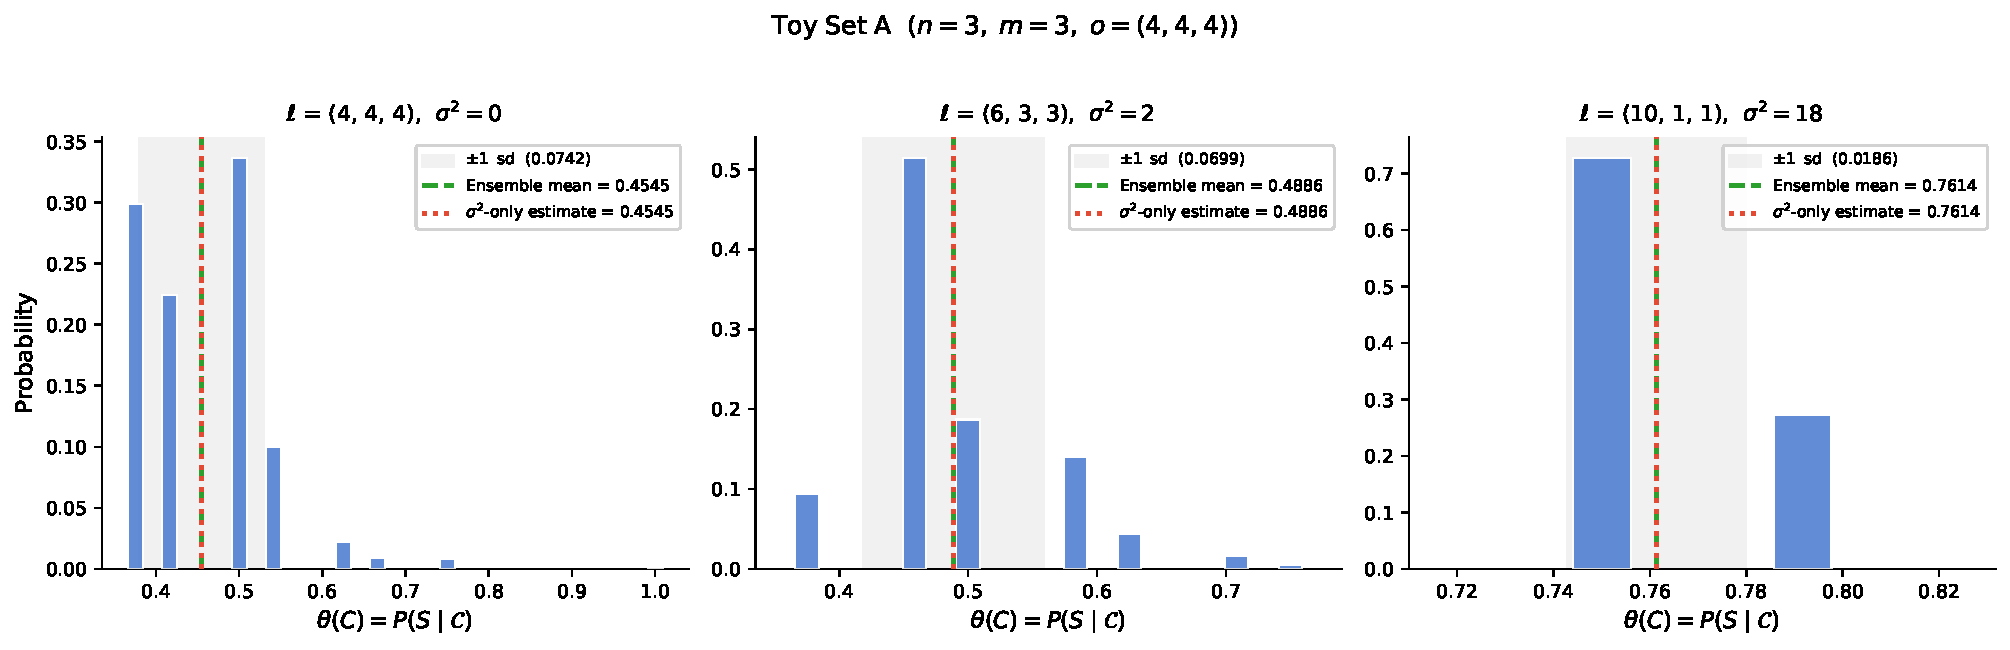
\includegraphics[width=\linewidth]{code/fig_toyA_hist.pdf}
\caption{Toy Set A ($n=3$, $m=3$, $o=(4,4,4)$): exact weighted distribution of $\theta(C)$ across all feasible contingency tables $C$ with margins $(\ell,o)$.
The dashed line marks the ensemble mean; the dotted line marks the $\sigma^2$-only point estimate (Theorem~\ref{thm:mean})---they coincide exactly.
The shaded band shows $\pm 1$ sd (Theorem~\ref{thm:var}).}
\label{fig:toyA-hist}
\end{figure}

\begin{figure}[htbp]
\centering
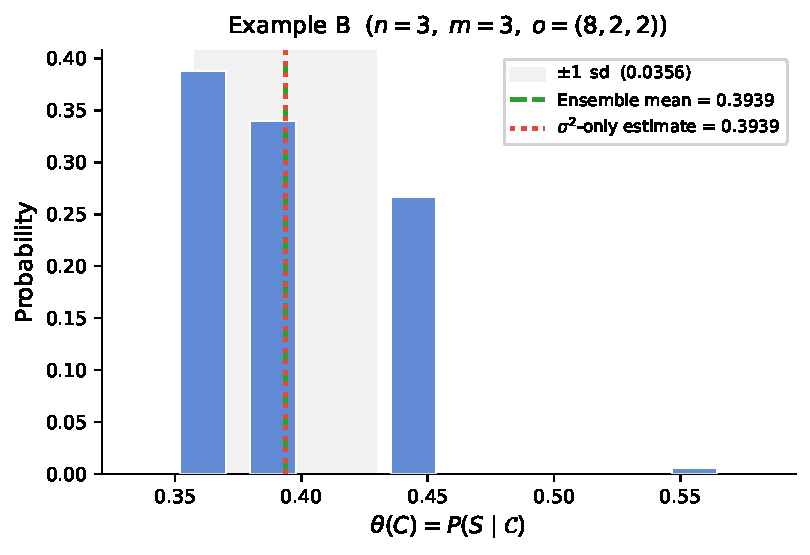
\includegraphics[width=0.55\linewidth]{code/fig_toyB_hist.pdf}
\caption{Toy Set B ($n=3$, $m=3$, $o=(8,2,2)$, $\ell=(4,4,4)$): exact weighted distribution of $\theta(C)$.
Dashed line: ensemble mean; dotted line: $\sigma^2$-only estimate (Theorem~\ref{thm:mean}); shaded band: $\pm 1$ sd (Theorem~\ref{thm:var}).}
\label{fig:toyB-hist}
\end{figure}

% ============================================================
\section{Choosing the entity-degree variance in practice}
\label{sec:sigma}

The estimator requires $\sigma^2$ (equivalently $\alpha$), which encodes heterogeneity of emission volume across entities.

\paragraph{Feasible range (active emitters).}
Because $\ell_i\ge 1$ and $\sum_i \ell_i=T$, not all $\sigma^2$ are possible.
Let $T=qn+r$ with $0\le r<n$.
Then:
\[
\sigma^2_{\min} = \frac{r(n-r)}{n^2}
\quad\text{(degrees as equal as possible, by a standard exchange argument)},
\]
\[
\sigma^2_{\max} = \frac{(n-1)(T-n)^2}{n^2}
\quad\text{(one dominant emitter, all others at 1)}.
\]

\paragraph{How to set $\sigma^2$ in practice.}
The primary recommendation is to set $\sigma^2$ from domain knowledge about the emission process, then verify robustness with a sensitivity sweep.

\smallskip\noindent\textbf{Domain elicitation (recommended).}
In many entity-resolution settings the analyst already knows, at least qualitatively, how heterogeneous emission volumes are.
For example, consider linking records on first names, where each person (entity) may appear under one or several given names (values).
Census and administrative data consistently show that most individuals use a single first name while a smaller fraction use two or more (due to cultural naming conventions, nicknames, or legal name changes).
This skewed-but-bounded pattern implies a moderate $\sigma^2$: well above the uniform baseline $\sigma^2\approx 0$, but far below the ``one dominant emitter'' extreme.
Translating even this rough qualitative knowledge into a plausible range for $\sigma^2$ is typically sufficient, because $\widehat\theta$ varies smoothly and monotonically in $\sigma^2$.

\smallskip\noindent\textbf{Variance-only sufficiency.}
Theorem~\ref{thm:mean} implies that $\widehat\theta$ depends on the entity-degree sequence $\ell$ only through $\sigma^2$: two degree sequences with different shapes but the same variance yield the same point estimate.
Figure~\ref{fig:ell-shapes} verifies this empirically.
Three hand-constructed $\ell$ vectors---spread, moderate, and peaked---all have $\sigma^2=36$ but very different higher moments ($M_3$ ranges from $16\,920$ to $22\,680$).
The MC distributions of $\theta(C)$ all centre on the same Theorem~\ref{thm:mean} estimate (dashed line).
The spread of each histogram differs (consistent with the $M_3$-dependence in Theorem~\ref{thm:var}), but the mean is invariant.
This means the analyst need only specify a single scalar, not the full shape of $\ell$.

\begin{figure}[htbp]
\centering
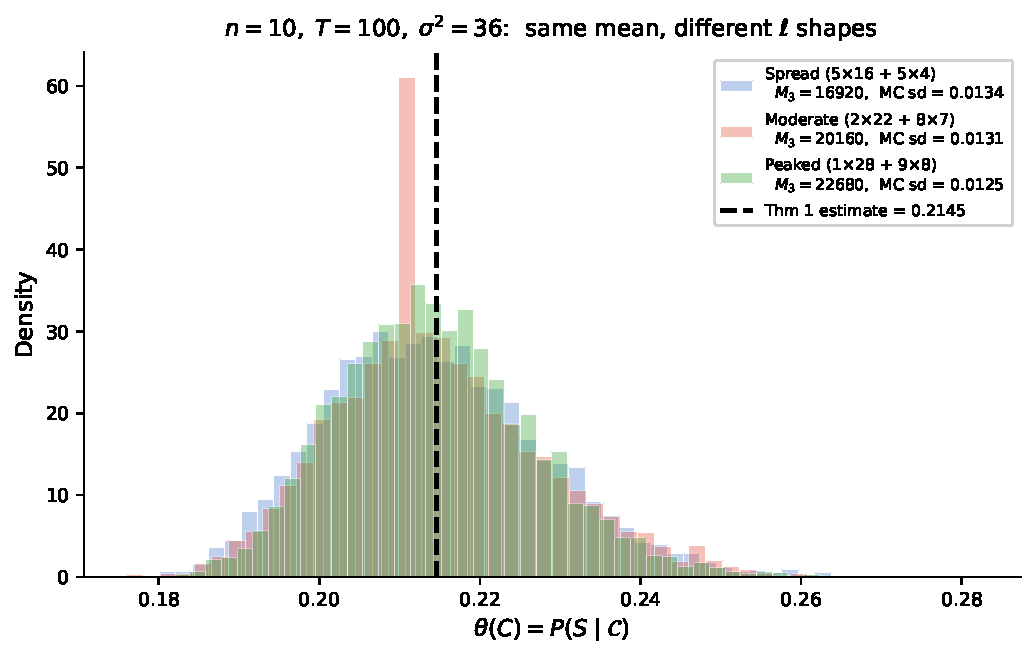
\includegraphics[width=0.75\linewidth]{code/fig_ell_shapes.pdf}
\caption{Three $\ell$ vectors with the same $\sigma^2=36$ but different shapes ($n=10$, $T=100$, uniform~$o$).
All three MC distributions centre on the Theorem~\ref{thm:mean} estimate (dashed), confirming that the mean depends on $\ell$ only through~$\sigma^2$.}
\label{fig:ell-shapes}
\end{figure}

\smallskip\noindent\textbf{Sensitivity analysis (robustness check).}
Given variance-only sufficiency, a sweep of $\widehat\theta$ over the feasible $\sigma^2$ interval fully characterises sensitivity.
The mapping $\sigma^2\mapsto\widehat\theta$ is monotone increasing, so a single plot immediately shows whether the conclusion depends on the heterogeneity assumption.

Figure~\ref{fig:sigma-sweep} demonstrates this for $n=20$, $m=15$, $T=200$ with two value marginals (uniform and Zipf-skewed).
The Theorem~\ref{thm:mean} curve (solid) sits inside the MC 5th--95th percentile band across the entire feasible range, confirming the formula at scale.
In both panels $\widehat\theta$ spans roughly $0.1$--$0.9$ over the full interval.
If domain knowledge places $\sigma^2$ in a narrow subinterval, the corresponding vertical slice gives tight bounds---the conclusion is robust.
If the plausible range maps to a wide band of $\widehat\theta$, the heterogeneity assumption matters and must be justified.

\begin{figure}[htbp]
\centering
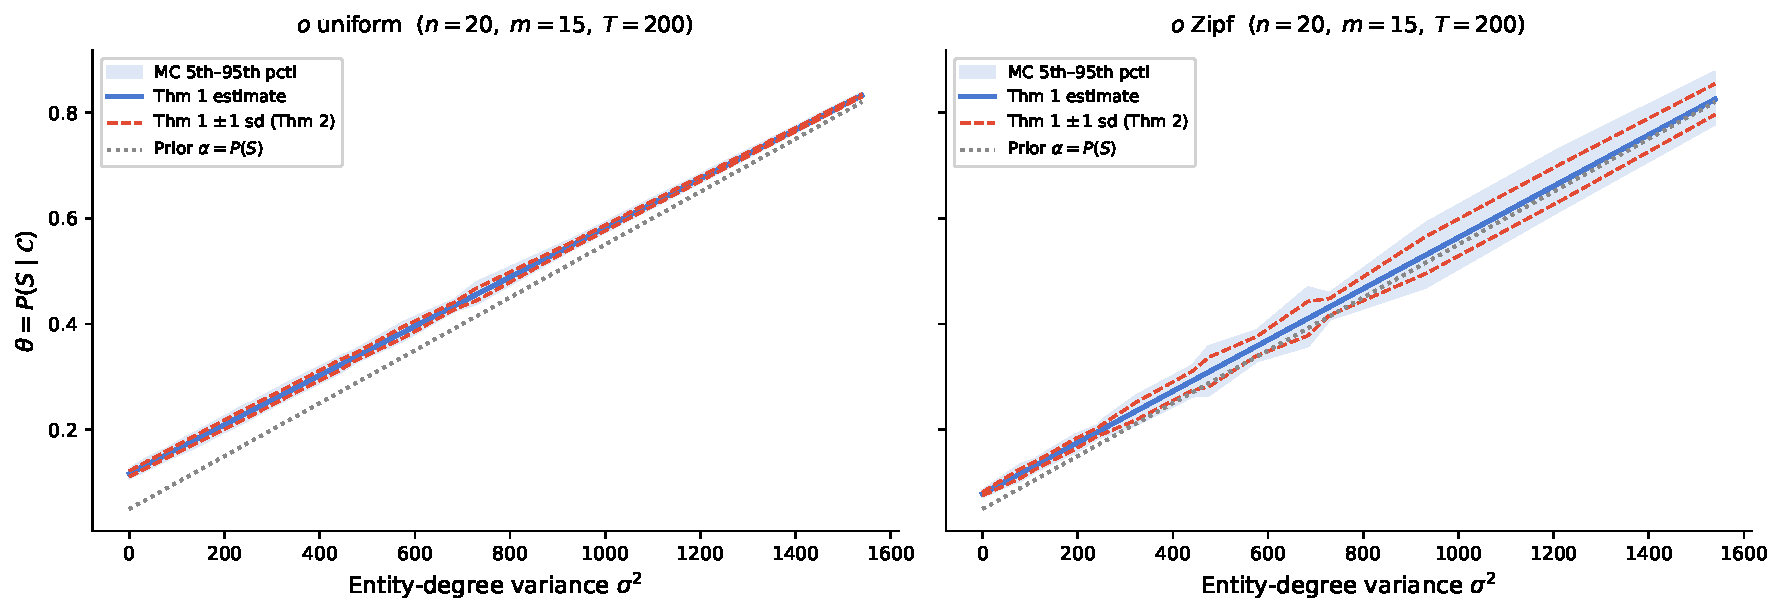
\includegraphics[width=\linewidth]{code/fig_sigma_sweep.pdf}
\caption{Sensitivity of $\widehat\theta$ to $\sigma^2$ for $n=20$, $m=15$, $T=200$.
Left: uniform $o$; right: Zipf-skewed $o$.
Solid line: Theorem~\ref{thm:mean}; shaded band: MC 5th--95th percentile ($B=500$); dashed lines: $\pm 1$ analytic sd (Theorem~\ref{thm:var}); grey dotted: prior $\alpha=P(S)$ (Section~\ref{sec:baselines}).}
\label{fig:sigma-sweep}
\end{figure}

\smallskip\noindent\textbf{Finite-sample estimation of value marginals.}
The preceding experiments assume that the value-degree vector $o$ is known exactly.
In practice, $o$ (equivalently, the marginal distribution $P(V{=}v_a)=o_a/T$) must be estimated from observed measurements.
To evaluate the impact of this estimation step, we run an end-to-end pipeline:
\begin{enumerate}[leftmargin=*]
\item Sample a ground-truth graph $C^*$ from the configuration model with specified $\ell$ and $o$.
\item Simulate $N_{\rm obs}$ single measurement draws from $C^*$ (each draw samples one edge uniformly and returns the value endpoint; the entity endpoint is latent and unobserved).
\item From the $N_{\rm obs}$ observed values, estimate the value-degree vector $\hat o$ by scaling empirical frequencies to the known total $T$.
\item Feed $(\hat o, n, \sigma^2)$ into the Theorem~\ref{thm:mean} estimator to obtain $\widehat\theta(\hat o)$.
\item Compare $\widehat\theta(\hat o)$ to both the oracle estimate $\widehat\theta(o)$ (which uses the true marginals) and the exact posterior $\theta(C^*)$ computed from the known graph.
\end{enumerate}

Figure~\ref{fig:demo-convergence} shows the result for three heterogeneity levels ($\sigma^2 = 0$, moderate, and high) using $n=20$, $m=15$, $T=200$ with uniform value marginals.
In each panel the blue curve and band show the median and 10th--90th percentile of $\widehat\theta(\hat o)$ over $R=300$ independent measurement simulations at each sample size $N_{\rm obs}$.
As $N_{\rm obs}$ grows, this band collapses onto the green dashed oracle line (the Theorem~\ref{thm:mean} estimate with true $o$), confirming that the finite-sample estimation error vanishes.
Convergence is effectively complete by $N_{\rm obs}\approx 500$--$1\,000$.

The red horizontal line marks the exact $\theta(C^*)$ for one specific ground-truth graph; the thin red lines show $\theta$ for eight additional sampled graphs.
All of these fall within the grey $\pm 1\,$sd ensemble band (Theorem~\ref{thm:var}), illustrating that the analytic uncertainty captures the graph-to-graph variation.
The gap between the oracle (green dashed) and any individual $\theta(C^*)$ (red) is the irreducible ensemble uncertainty: the estimator targets the ensemble mean, not the realization-specific posterior.

\begin{figure}[htbp]
\centering
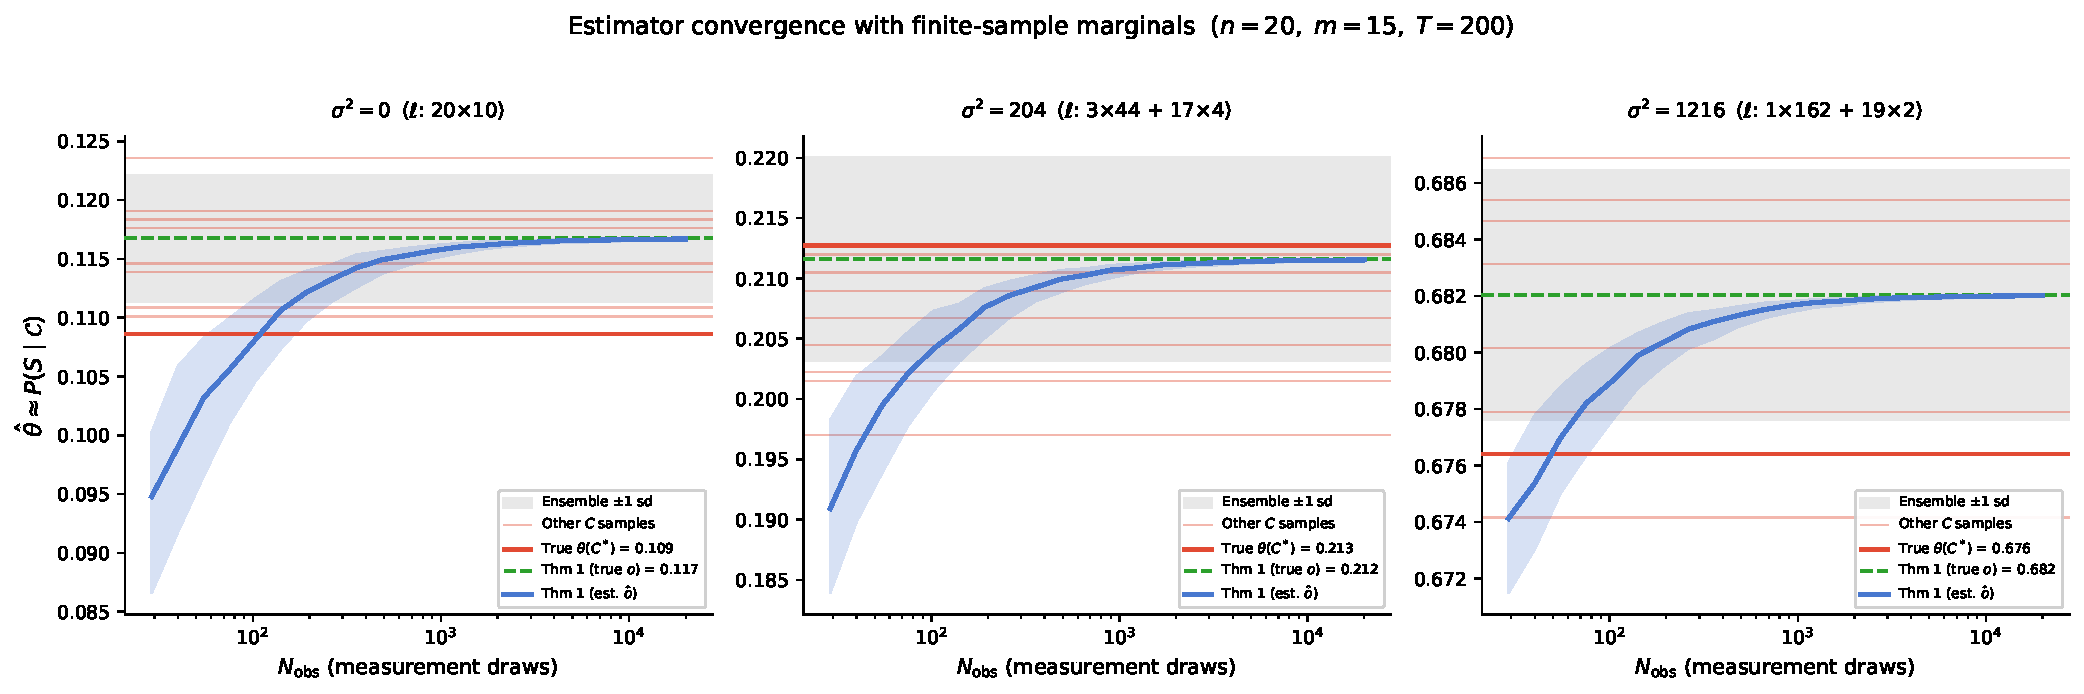
\includegraphics[width=\linewidth]{code/fig_demo_convergence.pdf}
\caption{Convergence of the Theorem~\ref{thm:mean} estimator when value marginals are estimated from finite data ($n=20$, $m=15$, $T=200$, uniform~$o$).
Each panel fixes one ground-truth graph $C^*$ at a different $\sigma^2$.
Blue curve/band: Theorem~\ref{thm:mean} estimate using $\hat o$ from $N_{\rm obs}$ simulated draws (median and 10th--90th percentile over 300 repetitions).
Green dashed: oracle estimate using true~$o$.
Red solid: exact $\theta(C^*)$; thin red lines: $\theta$ for eight other sampled graphs.
Grey band: $\pm 1\,$sd from Theorem~\ref{thm:var}.}
\label{fig:demo-convergence}
\end{figure}

\smallskip\noindent\textbf{Direct measurement-model validation.}
As a complementary check, we validate the measurement model end-to-end by simulating draw \emph{pairs} from a known graph $C^*$ and computing the empirical same-source rate among collisions.
For each pair, we draw two edges independently and uniformly from $C^*$, observe both the value endpoints (to detect a collision) and the entity endpoints (to check same-source status---information that would be latent in practice but is available in simulation).
The empirical estimator is
\[
\hat\theta_{\rm pairs} = \frac{\#\{\text{pairs with collision and same source}\}}{\#\{\text{pairs with collision}\}}.
\]
Figure~\ref{fig:demo-empirical} shows $\hat\theta_{\rm pairs}$ as a running average over 200\,000 simulated pairs for the moderate-$\sigma^2$ scenario.
The curve starts noisy (few collisions at small sample sizes, since the collision rate is ${\approx}\,6.7\%$) and converges to the exact $\theta(C^*)$ (red line), confirming that the algebraic formula $\theta(C)=\sum_{i,a}c_{ia}^2/\sum_a o_a^2$ correctly computes the same-source probability from the incidence matrix.

\begin{figure}[htbp]
\centering
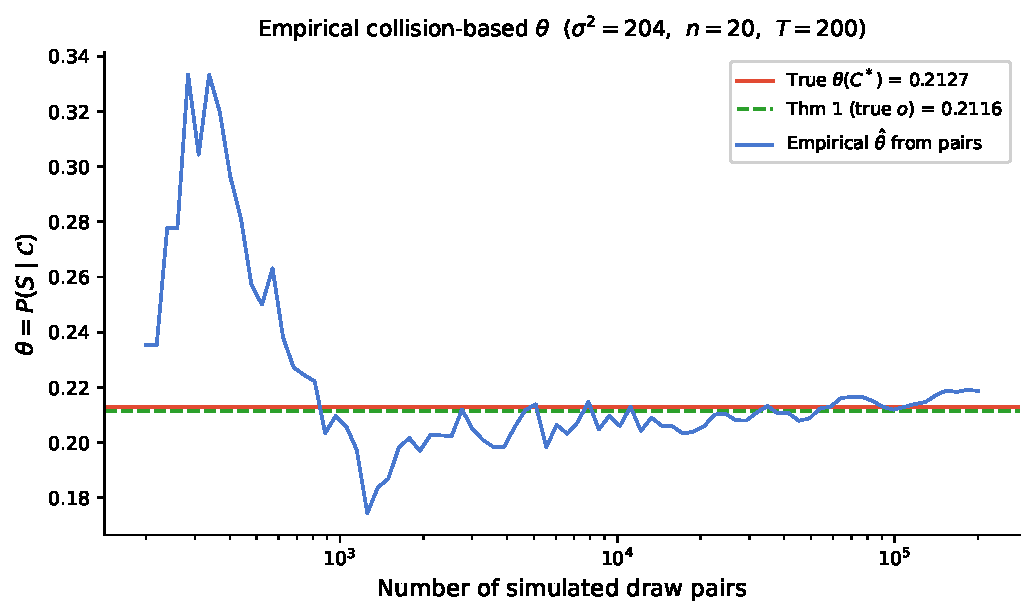
\includegraphics[width=0.6\linewidth]{code/fig_demo_empirical.pdf}
\caption{Direct measurement-model validation: empirical same-source rate among collisions from simulated draw pairs converges to the exact $\theta(C^*)$.
Red solid: exact $\theta(C^*)$; green dashed: Theorem~\ref{thm:mean} oracle estimate.
Blue curve: running empirical $\hat\theta_{\rm pairs}$ over 200\,000 pairs ($\sigma^2 \approx 204$, $n=20$, $T=200$).}
\label{fig:demo-empirical}
\end{figure}

% ============================================================
\section{Worked example: quasi-identifier collisions in event logs}
\label{sec:worked}

We illustrate the estimator on a synthetic-but-realistic scenario where entity identifiers are unavailable but domain knowledge about activity heterogeneity is available.

\paragraph{Setting.}
Consider a de-identified event log with $T=5{,}000$ rows, each generated by one of $n=100$ latent entities (users, devices, or patients).
Each row carries a quasi-identifier value (e.g., a demographic key such as \{age bracket, sex\} or a finer \{birth year, sex, ZIP3\}).
The analyst observes the value counts $o_1,\dots,o_m$ directly from the log and wants to estimate
\[
\theta = P(\text{same entity}\mid\text{same quasi-identifier value}).
\]
Operationally, $\theta$ is the precision of using quasi-identifier equality as a blocking key:
among all pairs of rows that agree on the key, what fraction correspond to the same underlying entity?

\paragraph{Inputs.}
The estimator (Algorithm~\ref{alg:mean}) requires:
(i)~the value counts~$o$ (computed directly from the log),
(ii)~the number of active entities~$n$, and
(iii)~a heterogeneity parameter~$\sigma^2$ describing the across-entity variance in activity volume.
In practice, $n$ and $\sigma^2$ come from domain knowledge, a privacy-safe aggregate report, or historical data from periods when stable identifiers were available.

\paragraph{Synthetic ground truth.}
To evaluate the estimator against a known answer, we generate entity activity volumes from a discretised lognormal distribution (log-space standard deviation $1.5$), producing heavy-tailed heterogeneity (median degree~$17$, maximum~$1{,}191$; resulting $\sigma^2\approx 16{,}841$).
We construct two quasi-identifier keys of different granularity:
\begin{itemize}[leftmargin=*]
\item \textbf{Coarse key} ($m=30$ distinct values, Zipf-distributed): collision rate $P(\coll)\approx 6.9\%$;
\item \textbf{Fine key} ($m=300$ distinct values, mildly skewed): collision rate $P(\coll)\approx 0.6\%$.
\end{itemize}
For each key, a ground-truth graph~$C^*$ is sampled from the configuration model with the generated degrees, giving exact posteriors $\theta(C^*)=0.083$ (coarse) and $\theta(C^*)=0.112$ (fine).

\paragraph{Results.}
Figure~\ref{fig:worked-example} shows the Theorem~\ref{thm:mean} estimate $\widehat\theta$ as a function of the assumed~$\sigma^2$ for both keys.
At the true $\sigma^2$, the estimator yields $\widehat\theta=0.080$ (coarse) and $\widehat\theta=0.110$ (fine), closely matching the ground truth.
Thin horizontal lines show $\theta$ for eight additional configuration-model graphs at the same degrees, confirming tight ensemble concentration.

Three practical conclusions emerge:
\begin{enumerate}[leftmargin=*]
\item \textbf{Key granularity matters.}
      The fine key has a ten-fold lower collision rate but collisions are more informative ($\theta\approx 0.11$ vs.\ $0.08$):
      when a fine-grained quasi-identifier repeats, it is more likely to be the same entity.
\item \textbf{Collision lift can be small for coarse keys.}
      The dotted prior curve $\alpha(\sigma^2)$ (Section~\ref{sec:baselines}) nearly coincides with the estimator for the coarse key,
      confirming that collisions on broad quasi-identifiers are barely more informative than the unconditional same-source rate.
      For the fine key, the gap between the prior and the estimator is substantially larger.
      This contrast is itself a useful diagnostic: the estimator quantifies \emph{how much} a collision adds beyond the prior, guiding the analyst toward keys where collisions carry real evidential weight.
\item \textbf{Heterogeneity matters.}
      Under the uniform-entity baseline ($\sigma^2\approx 0$), both estimates drop sharply ($\widehat\theta=0.013$ and $0.045$).
      The monotone $\sigma^2\mapsto\widehat\theta$ curve allows the analyst to read off how sensitive the conclusion is to the heterogeneity assumption.
\end{enumerate}

\begin{figure}[htbp]
\centering
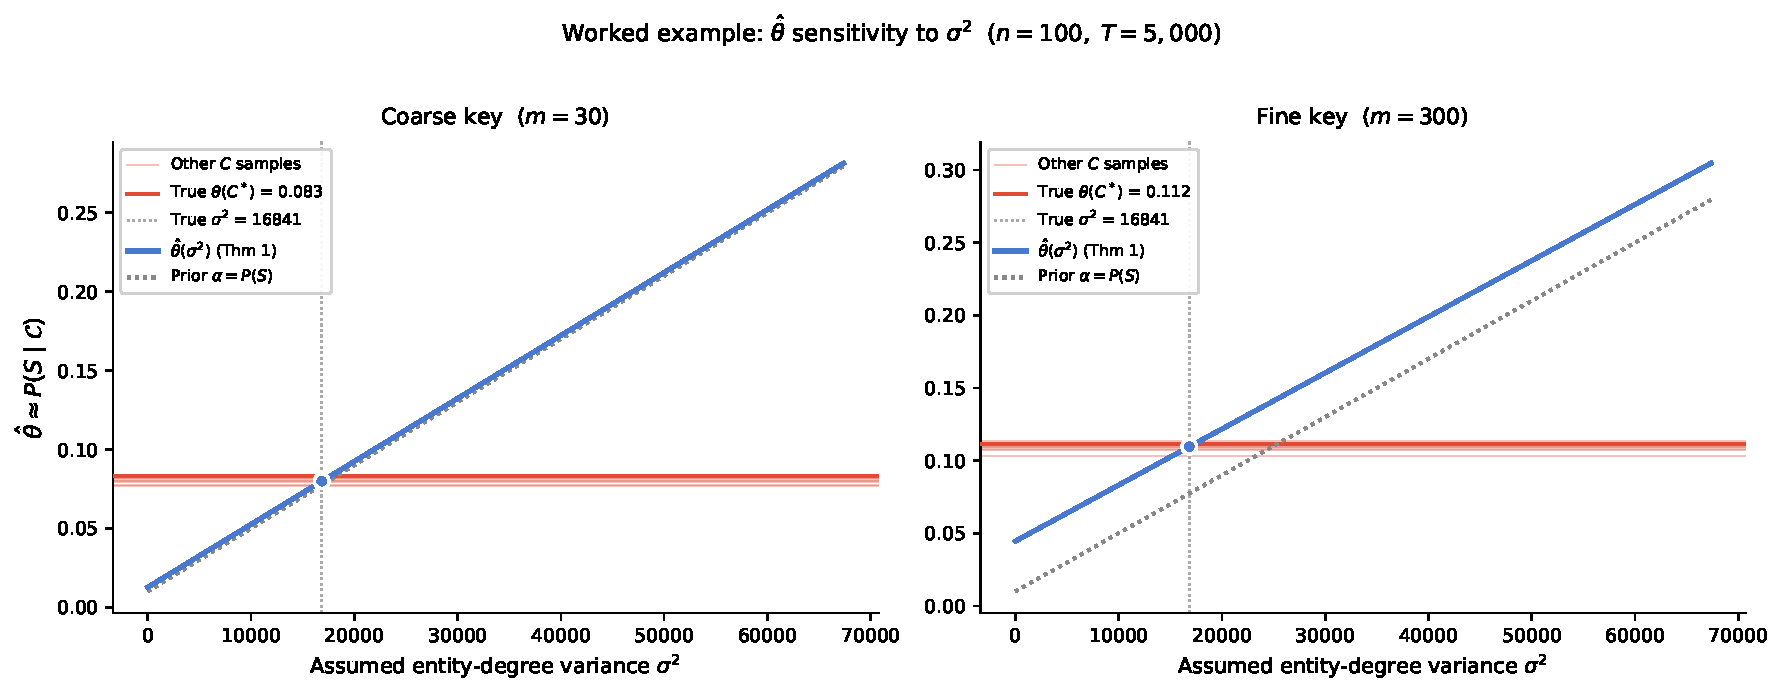
\includegraphics[width=\linewidth]{code/fig_worked_example.pdf}
\caption{Worked example ($n=100$, $T=5{,}000$): sensitivity of $\widehat\theta$ to assumed entity-degree variance~$\sigma^2$.
Left: coarse key ($m=30$); right: fine key ($m=300$).
Blue curve: Theorem~\ref{thm:mean} estimate.
Grey dotted: prior $\alpha=P(S)$ (Section~\ref{sec:baselines}); the gap is the collision lift.
Red line: exact $\theta(C^*)$; thin red lines: $\theta$ for eight additional sampled graphs.
Dotted vertical: true~$\sigma^2$.
Blue dot: $\widehat\theta$ at true~$\sigma^2$.}
\label{fig:worked-example}
\end{figure}

% ============================================================
\section{Discussion and conclusion}
\label{sec:discussion}

\subsection{Interpretation and limitations}

\paragraph{Why the mean is ``variance-only''.}
Theorem~\ref{thm:mean} shows that the ensemble mean depends on the entity side only through $M_2=\sum_i \ell_i(\ell_i-1)$, i.e., the degree second moment.
Thus a single heterogeneity parameter controls the mean estimate.

\paragraph{Sanity check connection.}
Proposition~\ref{prop:sanity} shows that $\alpha$ equals the \emph{unconditional} same-source probability $P(S)$.
The contribution of this paper is to characterize how conditioning on a collision $\coll$ transforms this baseline into $\E[\theta(C)\mid o,\alpha]$ under the configuration-model ensemble.

\paragraph{Why uncertainty needs more than variance.}
Theorem~\ref{thm:var} depends on $M_3=\sum_i \ell_i(\ell_i-1)(\ell_i-2)$, a skewness-sensitive statistic.
Therefore, a single variance parameter does not determine full uncertainty.
In practice, Monte Carlo bands under a chosen degree model are the most straightforward solution.

\paragraph{Modeling assumptions.}
The uniform-stub-matching (configuration-model) assumption is a principled default given degree information, but real systems may exhibit structure beyond degrees (e.g., specialization where certain entities preferentially emit certain values).
Such structure can shift $\theta(C)$ away from the configuration-model mean.
The toy distributions in Section~\ref{sec:toy} illustrate the spread even under the configuration model; structured deviations can be larger.

\paragraph{Finite-sample estimation of value marginals.}
The theoretical results assume that the value marginals $o$ (or $P(V{=}v_a)$) are known exactly.
In practice they are estimated from finite measurements.
Section~\ref{sec:sigma} demonstrates that the plug-in estimator $\widehat\theta(\hat o)$ converges to the oracle $\widehat\theta(o)$ with ${\approx}\,500$--$1\,000$ draws for the problem sizes tested.
A natural extension is to propagate sampling error analytically (e.g., via bootstrap over observed values or a Bayesian Dirichlet posterior over value probabilities) to quantify the additional uncertainty from marginal estimation.

\subsection{Future directions}

\paragraph{Value-conditioned collisions.}
A natural extension is to derive a closed-form expression for the configuration-model ensemble mean of
\[
P(S \mid V_1=V_2=v_a),
\]
i.e., the same-source posterior conditioned on a collision at a specific value label.
Such a result would provide a per-value ``collision informativeness'' statistic that complements the global collision event $\coll$.

\paragraph{Multi-field extensions.}
Record-linkage applications typically compare records on several fields simultaneously (e.g., name, date of birth, postal code), each governed by its own emission spectrum.
If fields are conditionally independent given the latent entity, the joint same-source posterior factorises into per-field contributions, and the present framework can be applied field by field.
When fields are correlated (e.g., name and ethnicity), a joint bipartite multigraph over field tuples is needed, and the configuration-model ensemble must respect cross-field dependence structure.
Characterising the ensemble mean of the joint posterior---and whether a tractable ``variance-only'' parameterisation survives---is an open question.
A related challenge is aggregating value-conditioned posteriors across multiple observed collisions to form a stronger overall same-source estimate, e.g., by treating per-collision posteriors as evidence factors in a probabilistic linkage objective.

\paragraph{Inverting collisions to estimate $\sigma^2$.}
This paper treats the entity-degree variance $\sigma^2$ as a domain-knowledge input.
A complementary direction is to \emph{estimate} $\sigma^2$ from observed data: if many pairs of draws are available, the empirical collision rate constrains $\alpha$ (and hence $\sigma^2$) via the relationship $P(\coll)=\sum_a (o_a/T)^2 \cdot \E[\theta(C)]$.
More generally, higher-order collision statistics (e.g., triple collisions) may identify additional degree-shape parameters such as $M_3$.
Formalising this inverse problem---including identifiability conditions and finite-sample rates---would make the framework fully data-driven.

\paragraph{Robustness beyond the configuration model.}
The configuration model is a maximum-entropy baseline, but real emission graphs may exhibit structure such as entity--value affinity (block structure) or degree--degree correlations (assortativity).
Quantifying how much such departures can shift $\theta(C)$ away from the configuration-model mean---e.g., via worst-case bounds over graphs with given marginals and bounded block structure---would provide robustness guarantees for practitioners.

\subsection{Concluding remarks}

We introduced a method for estimating the collision-conditioned same-source probability $P(S\mid \coll)$ in a latent-entity emission model when the full emission graph is unknown.
Under a maximum-entropy-over-matchings bipartite configuration-model ensemble consistent with observed value marginals, we proved that the ensemble mean of the exact posterior depends on the unknown entity side only through the entity-degree variance (second moment).
We also derived an analytic expression for ensemble variance across graphs, highlighting an additional dependence on degree skewness.
Small toy examples exactly enumerate the distribution of $\theta(C)$, validating the mean and variance formulas.
This yields a compact, interpretable framework: specify (or vary) a single heterogeneity parameter, compute a principled point estimate, and optionally quantify uncertainty via Monte Carlo or by specifying an additional skewness statistic.

% ============================================================
\appendix
\section{Proof of Theorem~\ref{thm:mean}}
\label{app:meanproof}

\begin{proof}
Fix $\ell$ and $o$.
For each entity $i$, consider its $\ell_i$ stubs.
After stub matching, each stub is assigned a value label; let $A(u)$ denote the label assigned to stub $u$.
Then the count of label $a$ in entity $i$ is $c_{ia}$, and
\[
\sum_{a=1}^m c_{ia}^2
=
\sum_{u,v \in i} \1\{A(u)=A(v)\}
=
\ell_i + \sum_{\substack{u,v\in i\\u\ne v}} \1\{A(u)=A(v)\}.
\]
Summing over $i$ yields
\[
N(C)=\sum_{i,a} c_{ia}^2 = T + X,
\quad
X := \sum_{\text{ordered within-entity pairs }(u,v),\,u\ne v}\1\{A(u)=A(v)\}.
\]
The number of ordered within-entity pairs is
\[
M_2=\sum_i \ell_i(\ell_i-1).
\]
Under uniform stub matching, for any ordered pair $(u,v)$ of distinct stubs, the probability that $A(u)=A(v)$ equals the probability that two distinct value stubs drawn uniformly without replacement share the same label:
\[
p_2 = \sum_a \frac{o_a}{T}\frac{o_a-1}{T-1}
= \frac{\sum_a \fall{o_a}{2}}{\fall{T}{2}}
= \frac{D-T}{T(T-1)}.
\]
Therefore $\E[X\mid \ell,o]=M_2 p_2$ and
\[
\E[N(C)\mid \ell,o] = T + M_2 p_2,
\qquad
\E[\theta(C)\mid \ell,o] = \frac{\E[N(C)\mid \ell,o]}{D} = \frac{T+M_2p_2}{D}.
\]
Finally, $M_2=\sum_i \ell_i(\ell_i-1)=\sum_i\ell_i^2 - T = T^2\alpha - T$, which yields the stated dependence on $\alpha$.
\end{proof}

\section{Proof of Theorem~\ref{thm:var}}
\label{app:varproof}

\begin{proof}
Write $X=\sum_{p\in \mathcal{P}} I_p$ where $\mathcal{P}$ is the set of ordered within-entity pairs $(u,v)$ with $u\ne v$, $|\mathcal{P}|=M_2$, and $I_p=\1\{A(u)=A(v)\}$.
Then $\theta(C)=(T+X)/D$, so $\Var(\theta)=\Var(X)/D^2$.

We compute $\Var(X)$ from second moments:
\[
\E[X^2] = \sum_{p} \E[I_p] + 2\sum_{p<q}\E[I_p I_q].
\]
For a fixed unordered pair $\{p,q\}$, there are three possible overlap types:
\begin{itemize}[leftmargin=*]
\item \textbf{Reverse pair:} $q$ is $(v,u)$ when $p$ is $(u,v)$. Joint probability is $p_2$.
There are exactly $M_2/2$ such unordered pairs.
\item \textbf{Share one stub:} $(u,v)$ and $(u,w)$, or $(v,u)$ and $(w,u)$, etc., involving three distinct stubs in the same entity. Joint probability is $p_3$.
For entity $i$, the number of unordered pairs of ordered pairs sharing one stub equals $2\fall{\ell_i}{3}$; summing gives $2M_3$.
\item \textbf{Disjoint:} four distinct stubs. Joint probability is $p_{22}$.
The remaining unordered pairs count is $\binom{M_2}{2} - \frac{M_2}{2} - 2M_3$.
\end{itemize}

Using $\E[I_p]=p_2$, we obtain:
\[
\E[X^2]
=
M_2 p_2
+ 2\Big[
\frac{M_2}{2}p_2 + (2M_3)p_3
+ \Big(\binom{M_2}{2} - \frac{M_2}{2} - 2M_3\Big)p_{22}
\Big].
\]
Algebra simplifies this to:
\[
\E[X^2] = 2M_2 p_2 + M_2(M_2-2)p_{22} + 4M_3(p_3-p_{22}).
\]
Since $\E[X]=M_2 p_2$, we have
\[
\Var(X) = \E[X^2] - (\E[X])^2
=
\Big(2M_2 p_2 + M_2(M_2-2)p_{22} + 4M_3(p_3-p_{22})\Big) - (M_2 p_2)^2.
\]
Dividing by $D^2$ gives Theorem~\ref{thm:var}.
\end{proof}

% ============================================================
\begin{thebibliography}{99}

\bibitem{simpson1949}
E.~H. Simpson.
\newblock Measurement of diversity.
\newblock \emph{Nature}, 163:688, 1949.

\bibitem{jaynes1957}
E.~T. Jaynes.
\newblock Information theory and statistical mechanics.
\newblock \emph{Physical Review}, 106(4):620--630, 1957.

\bibitem{parknewman2004}
J.~Park and M.~E.~J. Newman.
\newblock Statistical mechanics of networks.
\newblock \emph{Physical Review E}, 70(6):066117, 2004.

\bibitem{garlaschelli2008}
D.~Garlaschelli and M.~I. Loffredo.
\newblock Maximum likelihood: extracting unbiased information from complex networks.
\newblock \emph{Physical Review E}, 78(1):015101, 2008.

\bibitem{newman2010networks}
M.~E.~J. Newman.
\newblock \emph{Networks: An Introduction}.
\newblock Oxford University Press, 2010.

\bibitem{fosdick2018configuring}
D.~S. Fosdick, D.~B. Larremore, J.~Nishimura, and J.~Ugander.
\newblock Configuring the configuration model.
\newblock \emph{SIAM Review}, 60(2):315--355, 2018.

\bibitem{diaconisgangolli1995}
P.~Diaconis and A.~Gangolli.
\newblock Rectangular arrays with fixed margins.
\newblock In \emph{Discrete Probability and Algorithms} (Minneapolis, MN, 1993),
  Vol.~72 of \emph{IMA Volumes in Mathematics and its Applications},
  pages 15--41. Springer, 1995.

\bibitem{dyer1997}
M.~Dyer, R.~Kannan, and J.~Mount.
\newblock Sampling contingency tables.
\newblock \emph{Random Structures \& Algorithms}, 10:487--506, 1997.

\bibitem{chen2005smc}
Y.~Chen, P.~Diaconis, S.~Holmes, and J.~S. Liu.
\newblock Sequential {M}onte {C}arlo methods for statistical analysis of tables.
\newblock \emph{Journal of the American Statistical Association},
  100(469):109--120, 2005.

\bibitem{patefield1981}
W.~M. Patefield.
\newblock Algorithm {AS} 159: An efficient method of generating random $R \times C$
  tables with given row and column totals.
\newblock \emph{Applied Statistics}, 30(1):91--97, 1981.

\bibitem{diaconis1998algebraic}
P.~Diaconis and B.~Sturmfels.
\newblock Algebraic algorithms for sampling from conditional distributions.
\newblock \emph{The Annals of Statistics}, 26(1):363--397, 1998.

\bibitem{mosimann1962}
J.~E. Mosimann.
\newblock On the compound multinomial distribution, the multivariate $\beta$-distribution,
  and correlations among proportions.
\newblock \emph{Biometrika}, 49(1--2):65--82, 1962.

\bibitem{minka2000}
T.~P. Minka.
\newblock Estimating a {D}irichlet distribution.
\newblock Technical report, MIT, 2000.

\bibitem{fellegi1969}
I.~P. Fellegi and A.~B. Sunter.
\newblock A theory for record linkage.
\newblock \emph{Journal of the American Statistical Association}, 64(328):1183--1210, 1969.

\bibitem{jaro1989}
M.~A. Jaro.
\newblock Advances in record-linkage methodology as applied to matching the 1985 Census of {T}ampa, {F}lorida.
\newblock \emph{Journal of the American Statistical Association}, 84(406):414--420, 1989.

\bibitem{winkler2006}
W.~E. Winkler.
\newblock Overview of record linkage and current research directions.
\newblock Technical Report RR2006/02, U.S. Census Bureau, 2006.

\bibitem{copas1990}
J.~B. Copas and F.~J. Hilton.
\newblock Record linkage: Statistical models for matching computer records.
\newblock \emph{Journal of the Royal Statistical Society, Series A}, 153(3):287--312, 1990.

\bibitem{steorts2016}
R.~C. Steorts, R.~Hall, and S.~E. Fienberg.
\newblock A {B}ayesian approach to graphical record linkage and deduplication.
\newblock \emph{Journal of the American Statistical Association}, 111(516):1660--1672, 2016.

\bibitem{sadinle2017}
M.~Sadinle.
\newblock Bayesian estimation of bipartite matchings for record linkage.
\newblock \emph{Journal of the American Statistical Association}, 112(518):600--612, 2017.

\bibitem{flajolet1992birthday}
P.~Flajolet, D.~Gardy, and L.~Thimonier.
\newblock Birthday paradox, coupon collectors, caching algorithms, and self-organizing search.
\newblock \emph{Discrete Applied Mathematics}, 39(3):207--229, 1992.

\bibitem{sweeney2002}
L.~Sweeney.
\newblock $k$-anonymity: A model for protecting privacy.
\newblock \emph{International Journal of Uncertainty, Fuzziness and Knowledge-Based Systems}, 10(5):557--570, 2002.

\bibitem{narayanan2008}
A.~Narayanan and V.~Shmatikov.
\newblock Robust de-anonymization of large sparse datasets.
\newblock In \emph{IEEE Symposium on Security and Privacy}, pages 111--125, 2008.

\bibitem{elmagarmid2007}
A.~K. Elmagarmid, P.~G. Ipeirotis, and V.~S. Verykios.
\newblock Duplicate record detection: A survey.
\newblock \emph{IEEE Transactions on Knowledge and Data Engineering}, 19:1--16, 2007.

\bibitem{hernandez1995}
M.~A. Hern{\'a}ndez and S.~J. Stolfo.
\newblock The merge/purge problem for large databases.
\newblock In \emph{Proceedings of ACM SIGMOD}, pages 127--138, 1995.

\bibitem{christen2012book}
P.~Christen.
\newblock \emph{Data Matching: Concepts and Techniques for Record Linkage, Entity Resolution, and Duplicate Detection}.
\newblock Springer, 2012.

\bibitem{christen2012survey}
P.~Christen.
\newblock A survey of indexing techniques for scalable record linkage and deduplication.
\newblock \emph{IEEE Transactions on Knowledge and Data Engineering}, 24(9):1537--1555, 2012.

\bibitem{getoor2012}
L.~Getoor and A.~Machanavajjhala.
\newblock Entity resolution: theory, practice \& open challenges.
\newblock \emph{Proceedings of the VLDB Endowment}, 5(12):2018--2019, 2012.

\bibitem{bhattacharya2007}
I.~Bhattacharya and L.~Getoor.
\newblock Collective entity resolution in relational data.
\newblock \emph{ACM Transactions on Knowledge Discovery from Data}, 1(1):Article~5, 2007.

\end{thebibliography}

\end{document}

